%%%%%%%%%%%%%%%%%%%%%%%%%%%%%%%%%%%%%%%%%
% Programming/Coding Assignment
% LaTeX Template
%
% This template has been downloaded from:
% http://www.latextemplates.com
%
% Original author:
% Ted Pavlic (http://www.tedpavlic.com)
%
% Note:
% The \lipsum[#] commands throughout this template generate dummy text
% to fill the template out. These commands should all be removed when 
% writing assignment content.
%
% This template uses a Perl script as an example snippet of code, most other
% languages are also usable. Configure them in the "CODE INCLUSION 
% CONFIGURATION" section.
%
%%%%%%%%%%%%%%%%%%%%%%%%%%%%%%%%%%%%%%%%%

%----------------------------------------------------------------------------------------
%	PACKAGES AND OTHER DOCUMENT CONFIGURATIONS
%----------------------------------------------------------------------------------------

\documentclass[a4paper]{article}
\usepackage[utf8]{inputenc}
\usepackage{listingsutf8}
\usepackage[spanish]{babel}




\usepackage{fancyhdr} % Required for custom headers
\usepackage{lastpage} % Required to determine the last page for the footer
\usepackage{extramarks} % Required for headers and footers
\usepackage[usenames,dvipsnames]{color} % Required for custom colors
\usepackage{graphicx} % Required to insert images
\usepackage{listings} % Required for insertion of code
\usepackage{courier} % Required for the courier font
\usepackage{lipsum} % Used for inserting dummy 'Lorem ipsum' text into the template
\usepackage{svg}
\usepackage{attachfile}
\usepackage{currfile}
\usepackage{multicol}
\usepackage{alltt}
\usepackage{framed}
\usepackage{caption}
\usepackage{seqsplit}

\hypersetup{
colorlinks,
citecolor=black,
filecolor=black,
linkcolor=black,
urlcolor=blue
}


% Margins
\topmargin=-0.45in
\evensidemargin=0in
\oddsidemargin=0in
\textwidth=6.5in
\textheight=9.8in
\headsep=0.25in

\linespread{1.1} % Line spacing
\setlength{\parindent}{1.5em}
\setlength{\parskip}{1em}


% Set up the header and footer
\pagestyle{fancy}
%\lhead{\hmwkAuthorName} % Top left header
\lhead{\hmwkClass}
\rhead{\hmwkTitle} % Top right header
\chead{} % Top center head
\lfoot{\lastxmark} % Bottom left footer
\cfoot{} % Bottom center footer
\rfoot{ \thepage\ / \protect\pageref{LastPage}} % Bottom right footer
\renewcommand\headrulewidth{0.4pt} % Size of the header rule
\renewcommand\footrulewidth{0.4pt} % Size of the footer rule



%----------------------------------------------------------------------------------------
%	CODE INCLUSION CONFIGURATION
%----------------------------------------------------------------------------------------
\renewcommand{\ttdefault}{pcr}
\definecolor{MyDarkGreen}{rgb}{0.0,0.4,0.0} % This is the color used for comments
\lstloadlanguages{Perl} % Load Perl syntax for listings, for a list of other languages supported see: ftp://ftp.tex.ac.uk/tex-archive/macros/latex/contrib/listings/listings.pdf
\lstset{
language=sh, % Use Perl in this example
frame=single, % Single frame around code
basicstyle=\small\ttfamily, % Use small true type font
keywordstyle=[1]\small\color{Blue}\bf, % Perl functions bold and blue
keywordstyle=[2]\small\color{Purple}, % Perl function arguments purple
keywordstyle=[3]\small\color{Blue}\underbar, % Custom functions underlined and blue
identifierstyle=, % Nothing special about identifiers                                         
commentstyle=\small\color{MyDarkGreen}, % Comments small dark green courier font
stringstyle=\small\color{Purple}, % Strings are purple
showstringspaces=false, % Don't put marks in string spaces
tabsize=5, % 5 spaces per tab
morecomment=[l][\small\color{Blue}]{...}, % Line continuation (...) like blue comment
numbers=none, % Line numbers on left
firstnumber=1, % Line numbers start with line 1
numberstyle=\tiny\color{Blue}, % Line numbers are blue and small
stepnumber=0 % Line numbers go in steps of 5
}

% Creates a new command to include a perl script, the first parameter is the filename of the script (without .pl), the second parameter is the caption
\newcommand{\perlscript}[2]{
\begin{itemize}
\item[]\lstinputlisting[caption=#2,label=#1]{#1.pl}
\end{itemize}
}

%----------------------------------------------------------------------------------------
%	DOCUMENT STRUCTURE COMMANDS
%	Skip this unless you know what you're doing
%----------------------------------------------------------------------------------------

% Header and footer for when a page split occurs within a problem environment
\newcommand{\enterProblemHeader}[1]{
%\nobreak\extramarks{#1}{#1 continued on next page\ldots}\nobreak
%\nobreak\extramarks{#1 (continued)}{#1 continued on next page\ldots}\nobreak
}

% Header and footer for when a page split occurs between problem environments
\newcommand{\exitProblemHeader}[1]{
%\nobreak\extramarks{#1 (continued)}{#1 continued on next page\ldots}\nobreak
%\nobreak\extramarks{#1}{}\nobreak
}

\setcounter{secnumdepth}{0} % Removes default section numbers
\newcounter{homeworkProblemCounter} % Creates a counter to keep track of the number of problems

\newcommand{\homeworkProblemName}{}
\newenvironment{homeworkProblem}[1][]{ % Makes a new environment called homeworkProblem which takes 1 argument (custom name) but the default is "Problem #"
\stepcounter{homeworkProblemCounter} % Increase counter for number of problems
\renewcommand{\homeworkProblemName}{Ejercicio \arabic{homeworkProblemCounter} #1} % Assign \homeworkProblemName the name of the problem
\section{\homeworkProblemName} % Make a section in the document with the custom problem count
\enterProblemHeader{\homeworkProblemName} % Header and footer within the environment
}{
\exitProblemHeader{\homeworkProblemName} % Header and footer after the environment
%\clearpage
}


\newcommand{\problemAnswer}[1]{ % Defines the problem answer command with the content as the only argument
\noindent\framebox[\columnwidth][c]{\begin{minipage}{0.98\columnwidth}#1\end{minipage}} % Makes the box around the problem answer and puts the content inside
}

\newcommand{\homeworkSectionName}{}
\newenvironment{homeworkSection}[1]{ % New environment for sections within homework problems, takes 1 argument - the name of the section
\renewcommand{\homeworkSectionName}{#1} % Assign \homeworkSectionName to the name of the section from the environment argument
\subsection{\homeworkSectionName} % Make a subsection with the custom name of the subsection
\enterProblemHeader{\homeworkProblemName\ [\homeworkSectionName]} % Header and footer within the environment
}{
\enterProblemHeader{\homeworkProblemName} % Header and footer after the environment
}

%----------------------------------------------------------------------------------------
%	NAME AND CLASS SECTION
%----------------------------------------------------------------------------------------

\newcommand{\hmwkTitle}{Redefine el hmwkTitle} % Assignment title
\newcommand{\hmwkDueDate}{asdfadsf} % Due date
\newcommand{\hmwkClass}{Redefine hmwkClass} % Course/class
\newcommand{\hmwkClassTime}{} % Class/lecture time
\newcommand{\hmwkClassInstructor}{} % Teacher/lecturer
\newcommand{\hmwkAuthorName}{Álvaro González Sotillo} % Your name

%----------------------------------------------------------------------------------------
%	TITLE PAGE
%----------------------------------------------------------------------------------------

\title{
\vspace{2in}
\textmd{\textbf{\hmwkClass:\ \hmwkTitle}}\\
\vspace{0.1in}\large{\textit{\hmwkClassInstructor\ \hmwkClassTime}}
\vspace{3in}
}

\author{\textbf{\hmwkAuthorName}}
\date{} % Insert date here if you want it to appear below your name


%----------------------------------------------------------------------------------------

\usepackage{fancybox}
\newcommand{\codigo}[1]{\texttt{#1}}


% CUADRITO
\newsavebox{\fmboxx}
\newenvironment{cuadrito}[1][14cm]
{\noindent \begin{center} \begin{lrbox}{\fmboxx}\noindent\begin{minipage}{#1}}
{\end{minipage}\end{lrbox}\noindent\shadowbox{\usebox{\fmboxx}} \end{center}}





\newenvironment{entradasalida}[2][14cm]
{
  \newcommand{\elnombredelafiguradeentradasalida}{#2}
  \begin{figure}[h]
    \begin{cuadrito}[#1]
      \begin{scriptsize}
\begin{alltt}
}
{%
\end{alltt}%
      \end{scriptsize}%
    \end{cuadrito}%
    \caption{\elnombredelafiguradeentradasalida}
  \end{figure}
}


\newenvironment{entradasalidacols}[2][14cm]
{
\newcommand{\elnombredelafiguradeentradasalida}{#2}
%\begin{wrapfigure}{}{0.1}
\begin{cuadrito}[#1]
\begin{scriptsize}
\begin{alltt}
}
{
\end{alltt}
\end{scriptsize}
\end{cuadrito}
\captionof{figure}{\elnombredelafiguradeentradasalida}
%\end{wrapfigure}
}


\usepackage{pgffor}
\newcommand{\ficheroautoref}[0]{%
  \foreach \ficherotex in {../../../common/plantilla-ejercicio.tex,../../common/plantilla-ejercicio.tex,../common/plantilla-ejercicio.tex,../apuntes/common/plantilla-ejercicio.tex}{

    \IfFileExists{\ficherotex}%
    {%
      \textattachfile[mimetype=text/plain,%
      description={La plantilla},%
      subject={La plantilla}]%
      {\ficherotex}%
      {}%
      % RECUPERO ESPACIO VERTICAL PERDIDO
      \vspace{-6em}%
    }%
    {}%
  }
  

  \textattachfile[mimetype=text/plain,
  description={El fichero TEX original para crear este documento, no sea que se nos pierda},
  subject={El fichero TEX original para crear este documento, no sea que se nos pierda}]
  {\currfilename}{}

}

\newcommand{\entradausuario}[1]{\textit{\textbf{#1}}}

\newcommand{\enlace}[2]{\textcolor{blue}{{\href{#1}{#2}}}}

\newcommand{\adjuntarfichero}[3]{
\textattachfile[mimetype=text/plain,
color={0 0 0},
description={#3},
subject={#1}]
{#1}
{\textcolor{blue}{\codigo{#2}}}
}

\newcommand{\adjuntardoc}[2]{%
\textattachfile[mimetype=text/plain,%
color={0 0 0},%
description={#1},%
subject={#1}]%
{#1}%
{\textcolor{blue}{#2}}%
}%


\newcommand{\plantilladeclase}[2]{
\adjuntarfichero{#1.java}{#2}{Plantilla para la clase #2}
}

% https://en.wikibooks.org/wiki/LaTeX/Source_Code_Listings#Encoding_issue
\lstset{literate=
  {á}{{\'a}}1 {é}{{\'e}}1 {í}{{\'i}}1 {ó}{{\'o}}1 {ú}{{\'u}}1
  {Á}{{\'A}}1 {É}{{\'E}}1 {Í}{{\'I}}1 {Ó}{{\'O}}1 {Ú}{{\'U}}1
  {à}{{\`a}}1 {è}{{\`e}}1 {ì}{{\`i}}1 {ò}{{\`o}}1 {ù}{{\`u}}1
  {À}{{\`A}}1 {È}{{\'E}}1 {Ì}{{\`I}}1 {Ò}{{\`O}}1 {Ù}{{\`U}}1
  {ä}{{\"a}}1 {ë}{{\"e}}1 {ï}{{\"i}}1 {ö}{{\"o}}1 {ü}{{\"u}}1
  {Ä}{{\"A}}1 {Ë}{{\"E}}1 {Ï}{{\"I}}1 {Ö}{{\"O}}1 {Ü}{{\"U}}1
  {â}{{\^a}}1 {ê}{{\^e}}1 {î}{{\^i}}1 {ô}{{\^o}}1 {û}{{\^u}}1
  {Â}{{\^A}}1 {Ê}{{\^E}}1 {Î}{{\^I}}1 {Ô}{{\^O}}1 {Û}{{\^U}}1
  {œ}{{\oe}}1 {Œ}{{\OE}}1 {æ}{{\ae}}1 {Æ}{{\AE}}1 {ß}{{\ss}}1
  {ű}{{\H{u}}}1 {Ű}{{\H{U}}}1 {ő}{{\H{o}}}1 {Ő}{{\H{O}}}1
  {ç}{{\c c}}1 {Ç}{{\c C}}1 {ø}{{\o}}1 {å}{{\r a}}1 {Å}{{\r A}}1
  {€}{{\euro}}1 {£}{{\pounds}}1 {«}{{\guillemotleft}}1
  {»}{{\guillemotright}}1 {ñ}{{\~n}}1 {Ñ}{{\~N}}1 {¿}{{?`}}1
}

\lstset{
  inputencoding=utf8,
  captionpos=b,
  frame=single,
  basicstyle=\small\ttfamily,
  showstringspaces=false,
  numbers=none,
  numbers=left,
  xleftmargin=2em,
  breaklines=true,
  postbreak=\mbox{\textcolor{red}{$\hookrightarrow$}\space}
}

\renewcommand{\lstlistingname}{Listado}
\captionsetup[lstlisting]{font={footnotesize},labelfont=bf,position=bottom}
\captionsetup[figure]{font={footnotesize},labelfont=bf}
\lstnewenvironment{listadojava}[2]
{
  \lstset{language=Java,caption={#1},label={#2}}
  \noindent\minipage{\linewidth}%
}
{\endminipage}

% LISTADO SHELL
\lstnewenvironment{listadoshell}[2]
{
  \lstset{language=bash,caption={#1},label={#2}}
  \noindent\minipage{\linewidth}%
}
{\endminipage}

% LISTADO TXT
\lstnewenvironment{listadotxt}[2]
{
  \lstset{caption={#1},label={#2}, keywords={}}
  \noindent\minipage{\linewidth}%
}
{\endminipage}

% LISTADO SQL
\lstnewenvironment{listadosql}[2]%
{%
  %(el 1 )caption es #1\\%
  %(el 2) label es #2\\%
  \lstset{language=sql,caption={#1},label={#2}}%
  \noindent\minipage{\linewidth}%
}
{\endminipage}
  






\newcommand{\graficosvg}[3][14cm]{
\begin{figure}[htbp]
\centering
\textattachfile{#2.svg}{
\color{black}
\includesvg[width=#1]{#2}
}
\caption{#3}
\end{figure}
}


\newcommand{\graficosvguml}[3][7cm]{
  \texttt{\graficosvg[#1]{#2}{#3}}
}


\newcommand{\primerapagina}{
\newpage
\ficheroautoref
\tableofcontents
\newpage
}

% CAJAS
\usepackage[skins]{tcolorbox}
\newtcolorbox{Aviso}[1][Aviso]{
  enhanced,
  colback=gray!5!white,
  colframe=gray!75!black,fonttitle=\bfseries,
  colbacktitle=gray!85!black,
  attach boxed title to top left={yshift=-2mm,xshift=2mm},
  title=#1
}


\newcommand{\StudentData}{
  \begin{cuadrito}[1\textwidth]
    \vspace{0.3cm}
    \large{
      \textbf{Apellidos:} \hrulefill \\
      \textbf{Nombre:} \hrulefill \\
      \textbf{Fecha:} \hrulefill \hspace{1cm} \textbf{Grupo:} \hrulefill \\
    }
    %\vspace{0.2cm}
  \end{cuadrito}
}

% TEXTO EN MONOESPACIO PERO QUE SE PARTE EN LINEAS
\usepackage{seqsplit}
\newcommand{\tecnico}[1]{\texttt{\seqsplit{#1}}}

% REEMPLAZAR TEXTO, NO LO USO
\def\replace#1#2#3{%
 \def\tmp##1#2{##1#3\tmp}%
   \tmp#1\stopreplace#2\stopreplace}
\def\stopreplace#1\stopreplace{}

\usepackage{eurosym}


\renewcommand{\hmwkClass}{Planificación y Administración de Redes}
\renewcommand{\hmwkTitle}{Práctica de conexiones TCP}




\begin{document}

% \maketitle

% ----------------------------------------------------------------------------------------
%	TABLE OF CONTENTS
% ----------------------------------------------------------------------------------------

% \setcounter{tocdepth}{1} % Uncomment this line if you don't want subsections listed in the ToC

\primerapagina

\setlength{\parindent}{0em}
\setlength{\parskip}{1em}


\section{Objetivo de la práctica}
Los objetivos  de la práctica son:
\begin{itemize}
\item Familiarizarse con los conceptos de puerto y conexión
\item Implementar NAT
\item Exponer servicios a través de un NAT  
\item Manejar conexiones de ISP y routers SOHO
\end{itemize}


La última versión de esta práctica está disponible en \enlace{https://alvarogonzalezsotillo.github.io/apuntes-clase/planificacion-administracion-redes-asir1/apuntes/6/par-6-practica-nat-desde-casa.pdf}{este enlace}.


\section{Preparación del entorno}
\begin{itemize}
\item Máquina virtual Linux (recomendado Debian)
  \begin{itemize}
  \item No necesita mucha memoria (256 MBytes)
  \item Tendrá una tarjeta de red \textit{bridged} con una dirección en la red local de casa (generalmente \texttt{192.168.0.0/24} o \texttt{192.168.1.0/24}). Se sugiere que sea la última libre, y en el resto de la práctica se supondrá que es \texttt{192.168.1.254/24}.
  \item Tendrá una tarjeta de red \textit{host only}, para poder comunicarse con ella aunque falle la conexión real 
  \end{itemize}

\item Máquina virtual Windows, versión \textit{profesional}, \textit{ultimate} o equivalente (las que permitan \enlace{https://www.redeszone.net/2016/01/30/activar-escritorio-remoto-windows-10-8-1-7/}{Escritorio Remoto})
  \begin{itemize}
  \item No necesita mucha memoria (512 MBytes)    
  \item Tendrá una tarjeta de red \textit{bridged} con una dirección en la red local de casa. Se sugiere que sea la penúltima libre, y en el resto de la práctica se supondrá que es \texttt{192.168.1.253/24}.
  \item Tendrá una tarjeta de red \textit{host only}, para poder comunicarse con ella aunque falle la conexión real 
  \end{itemize}
\end{itemize}

No se recomienda utilizar ordenadores reales directamente, para mejorar la seguridad.

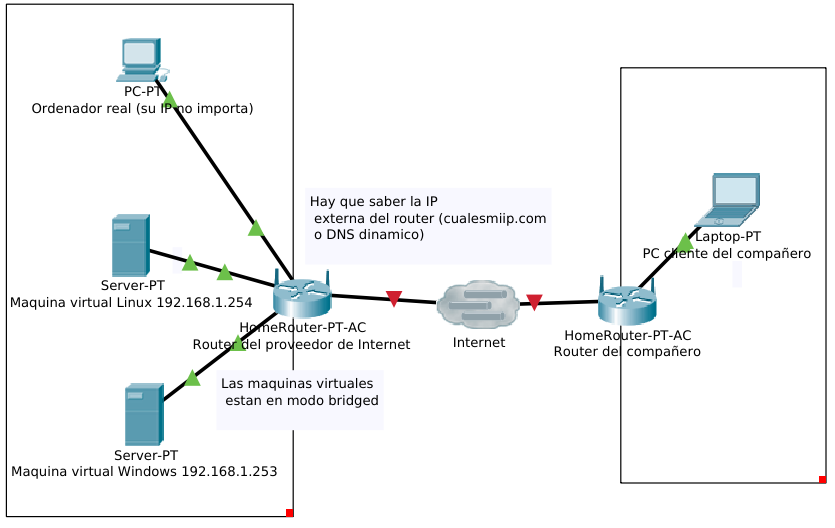
\includegraphics[width=\textwidth]{./media/practica-nat-en-casa.png}


\begin{homeworkProblem}[: \imenu{Registra tu dirección IP real en Internet}]
  \begin{itemize}
  \item Los ISP generalmente no dan direcciones fijas en Internet.
  \item Tu router tendrá una dirección externa obtenida por DHCP, que puede cambiar en cualquier momento
  \item Para saber cuál es tu dirección en Internet puedes
    \begin{itemize}
    \item Consultar páginas como \url{http://www.cualesmiip.com/}. Deberás consultarla cada poco tiempo, por si tu IP cambia
    \item Registrarte en un \enlace{https://www.ionos.es/digitalguide/servidores/know-how/que-es-un-dyndns-dns-dinamico/}{DNS dinámico} gratuito, como \url{https://www.noip.com/}
    \end{itemize}
  \end{itemize}
\end{homeworkProblem}

\begin{homeworkProblem}[: Comprueba la conectividad de las máquinas virtuales]
  \begin{itemize}
  \item Asigna a las máquinas virtuales las direcciones indicadas
    
  \item Comprueba que pueden accederse entre sí (con \texttt{ping}) y que tienen conexión a Internet.
  \end{itemize}
\end{homeworkProblem}

\begin{homeworkProblem}[: Abre un puerto a la máquina virtual Linux]
  \begin{itemize}
  \item Instala el servidor ssh, con \texttt{sudo apt-get install openssh-server}. Observa con \texttt{netstat -antp} que el servicio sshd está en el puerto \texttt{22}.
  \item Si no tienes un usuario no \texttt{root}, crea uno con \texttt{sudo adduser remoto}
  \item En el router de tu ISP abre el puerto \texttt{222}, y conéctalo al puerto \texttt{22} de la máquina virtual Linux
    \begin{itemize}
    \item Del puerto extero \texttt{222} a la dirección \texttt{192.168.1.254}, puerto \texttt{22}
    \item Cada router es distinto. Si tienes problemas contacta con el profesor.
    \end{itemize}
  \end{itemize}

  \begin{Aviso}
    No se recomienda abrir el puerto \texttt{22} en el router, ya que muchos bots de Internet intentan continuamente entrar por ese puerto. El puerto \texttt{222} es mucho más tranquilo. 
  \end{Aviso}
\end{homeworkProblem}


\begin{homeworkProblem}[: \imenu{Pide a un compañero que se conecte a tu servidor linux}]
  \begin{itemize}
  \item Pásale a un compañero tu IP (o nombre de dominio registrado en un DNS dinámico), el nombre de usuario y la contraseña de linux. Si el puerto que has abierto en el router no es el \texttt{222}, comunícaselo también.
  \item El compañero se conectará con un cliente SSH
    \begin{itemize}
    \item Desde windows: \enlace{https://mobaxterm.mobatek.net/}{MobaXterm}, \enlace{https://putty.org/}{PuTTY}
    \item Desde linux: En la línea de comandos, \texttt{ssh usuario@DIRECCIONIPEXTERNADELROUTER -p 222}
    \end{itemize}
    
  \item Para demostrar que se ha conectado a tu ordenador, el compañero creará un directorio con su nombre: \texttt{mkdir manolo-ha-estado-aqui}
  \item Puedes monitorizar con el comando \texttt{who} para ver quién está conectado en cada momento.
  \end{itemize}
  
\end{homeworkProblem}


\begin{homeworkProblem}[: \imenu{Abre un puerto a la máquina virtual Windows}]
  \begin{itemize}
  \item Habilita las conexiones por escritorio remoto a tu máquina virtual Windows: \url{https://www.redeszone.net/2016/01/30/activar-escritorio-remoto-windows-10-8-1-7/}. Observa con \texttt{netstat} que el servicio está escuchando en el puerto \texttt{3389}.
  \item En el router de tu ISP abre el puerto \texttt{33389}, y conéctalo al puerto \texttt{3389} de la máquina virtual Windows
    \begin{itemize}
    \item Del puerto extero \texttt{33389} a la dirección \texttt{192.168.1.253}, puerto \texttt{3389}
    \item Cada router es distinto. Si tienes problemas contacta con el profesor.
    \end{itemize}
  \end{itemize}

  \begin{Aviso}
    No se recomienda abrir el puerto \texttt{3389} en el router, ya que muchos bots de Internet intentan continuamente entrar por ese puerto. El puerto \texttt{33389} es mucho más tranquilo. 
  \end{Aviso}
\end{homeworkProblem}


\begin{homeworkProblem}[: \imenu{Pide a un compañero que se conecte a tu servidor Windows}]
  \begin{itemize}
  \item Pásale a un compañero tu IP (o nombre de dominio registrado en un DNS dinámico), el nombre de usuario y la contraseña de windows. Si el puerto que has abierto en el router no es el \texttt{33389}, comunícaselo también.
  \item El compañero se conectará con el cliente Remote Desktop
    \begin{itemize}
    \item Desde windows: Ejecuta en el terminal \texttt{mstsc /v:DIRECCIONIPEXTERNADELROUTER:33389}
      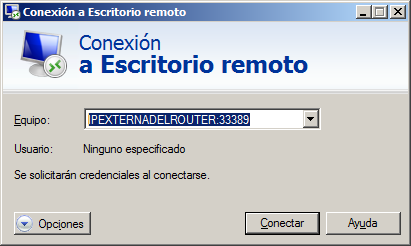
\includegraphics{./media/conexion-con-mstsc.png}
    \item Desde linux: Lo mejor es instalar y usar \enlace{https://remmina.org/how-to-install-remmina/}{remmina}.
    \end{itemize}
  \item Windows te pedirá confirmación para que tu compañero tome el control de la máquina virtual. En las versiones no servidor de Windows \enlace{http://woshub.com/how-to-allow-multiple-rdp-sessions-in-windows-10/}{solo una persona puede controlar el ordenador} a la vez.  
  \item Para demostrar que se ha conectado a tu ordenador, el compañero creará un directorio con su nombre en el escritorio
  \end{itemize}
  
\end{homeworkProblem}


\section{Conclusión}

Se puede realizar esta práctica con cualquier otro servicio (páginas web, carpetas compartidas...). Basta con saber el número de puerto correspondiente a ese servicio.

\end{document}
